\documentclass[10pt,letterpaper]{article}
\usepackage[letterpaper, margin=0.5in]{geometry}
\usepackage{tikz}
\usepackage{ifthen}

\begin{document}

\par\noindent
Goal:\break
\includegraphics[width=0.5\linewidth]{reference_images/abs_graph.png}

\par\noindent
TikZ:\break
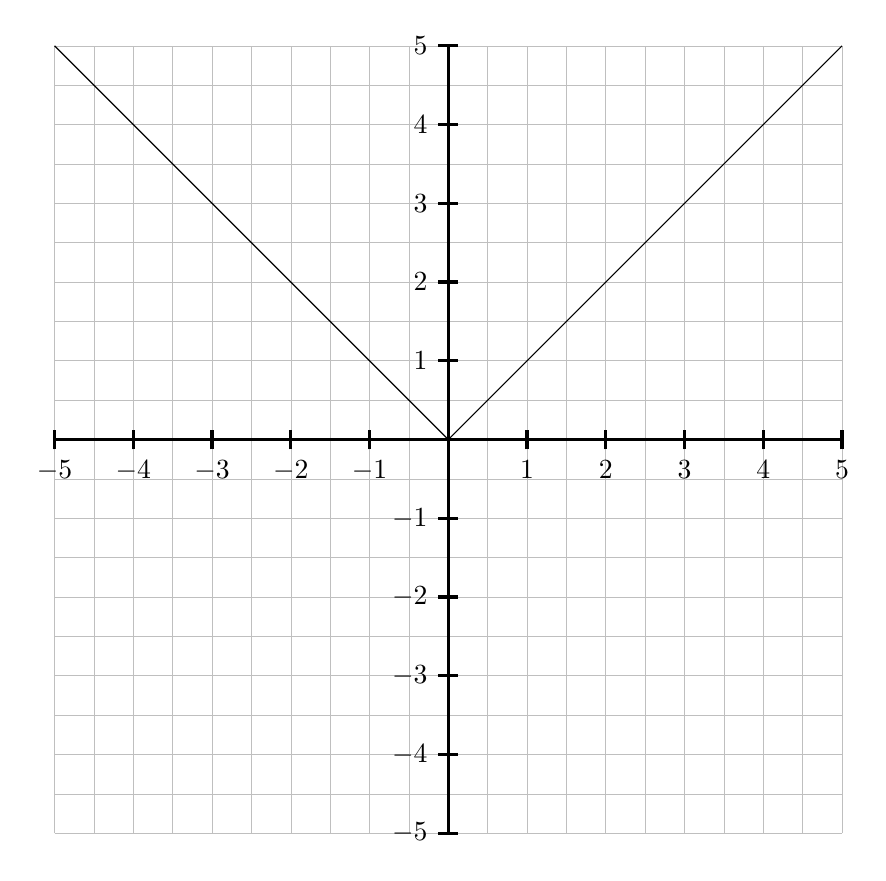
\begin{tikzpicture}
	% Coordinate grid
	\draw[step=0.5, very thin, lightgray] (-5,-5) grid (5,5);

	% Coordinate axes
	\draw[very thick] (-5,0) -- (5,0);
	\draw[very thick] (0,-5) -- (0,5);

	% Draw the function
	\draw (-5,5) -- (0,0) -- (5,5);

	% Stylize coordinate axes
	\foreach \x in {-5,...,5} {
		\draw[very thick] (\x,-0.125) node[anchor=north]{$\ifthenelse{\x=0}{}{\x}$} -- (\x,0.125);
		\draw[very thick] (-0.125,\x) node[anchor=east]{$\ifthenelse{\x=0}{}{\x}$} -- (0.125,\x);
	}
\end{tikzpicture}

\newpage
\par\noindent
Goal:\break
\includegraphics[width=0.75\linewidth]{reference_images/pythagorean_theorem.png}

\par\noindent
TikZ:\break
% First shape
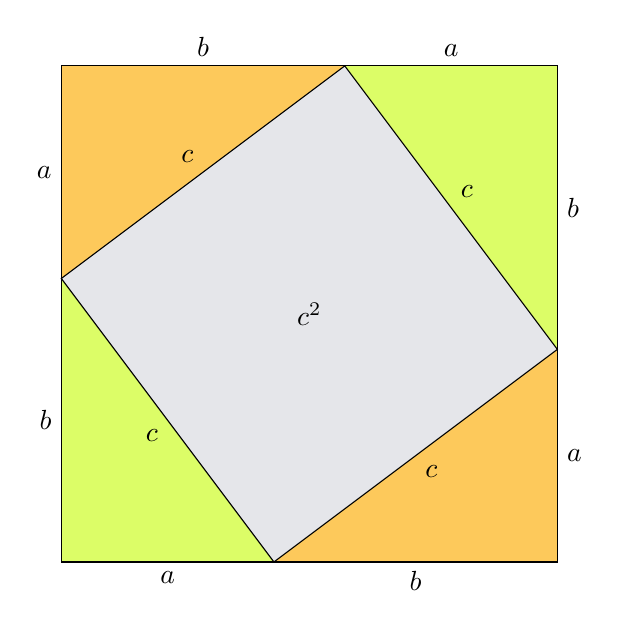
\begin{tikzpicture}[scale=0.9]
	% Shading
	\fill[fill={rgb,255:red,220;green,253;blue,103}] (0,0) -- (3,0) -- (0,4) -- cycle;
	\fill[fill={rgb,255:red,220;green,253;blue,103}] (7,7) -- (4,7) -- (7,3) -- cycle;
	\fill[fill={rgb,255:red,253;green,201;blue,91}] (3,0) -- (7,0) -- (7,3) -- cycle;
	\fill[fill={rgb,255:red,253;green,201;blue,91}] (0,7) -- (0,4) -- (4,7) -- cycle;
	\fill[fill={rgb,255:red,229;green,230;blue,234}] (3,0) -- (7,3) -- (4,7) -- (0,4) -- cycle;
	% Lines
	\draw[thin] (0,0) -- (7,0) -- (7,7) -- (0,7) -- (0,0);
	\draw (3,0) -- (7,3) -- (4,7) -- (0,4) -- (3,0);
	% Labels
	\draw (3.5,3.5) node {$c^2$};
	\draw (1.5,0) node[anchor=north] {$a$};
	\draw (5,0) node[anchor=north] {$b$};
	\draw (2,7) node[anchor=south] {$b$};
	\draw (5.5,7) node[anchor=south] {$a$};
	\draw (0,2) node[anchor=east] {$b$};
	\draw (0,5.5) node[anchor=east] {$a$};
	\draw (7,1.5) node[anchor=west] {$a$};
	\draw (7,5) node[anchor=west] {$b$};
	\draw (1.5,2) node[anchor=north east] {$c$};
	\draw (5,1.5) node[anchor=north west] {$c$};
	\draw (5.5,5) node[anchor=south west] {$c$};
	\draw (2,5.5) node[anchor=south east] {$c$};
\end{tikzpicture}
% Second shape
\hspace{1cm}
\definecolor{mygreen}{RGB}{220,253,103}
\definecolor{myorange}{RGB}{253,201,91}
\definecolor{mygray}{RGB}{229,230,234}
\begin{tikzpicture}[scale=0.9]
	% Shading
	\fill[fill=mygray] (0,0) -- (0,7) -- (7,7) -- (7,0) -- cycle;
	\fill[fill=mygreen] (0,7) -- (0,3) -- (3,3) -- (3,7) -- cycle;
	\fill[fill=myorange] (3,0) -- (7,0) -- (7,3) -- (3,3) -- cycle;
	% Lines
	\draw[thin] (0,0) -- (7,0) -- (7,7) -- (0,7) -- (0,0);
	\draw (0,3) -- (7,3);
	\draw (3,0) -- (3,7);
	\draw (0,7) -- (3,3);
	\draw (3,0) -- (7,3);
	% Labels
	\draw (1.5,1.5) node {$a^2$};
	\draw (5,5) node {$b^2$};
	\draw (1.5,0) node[anchor=north] {$a$};
	\draw (1.5,7) node[anchor=south] {$a$};
	\draw (0,1.5) node[anchor=east] {$a$};
	\draw (7,1.5) node[anchor=west] {$a$};
	\draw (5,0) node[anchor=north] {$b$};
	\draw (5,7) node[anchor=south] {$b$};
	\draw (0,5) node[anchor=east] {$b$};
	\draw (7,5) node[anchor=west] {$b$};
\end{tikzpicture}

\end{document}